\chapter{THEORETICAL BACKGROUND AND LITERATURE REVIEW}
\onehalfspacing
\label{chap:literature-review}
\vspace{-3em}
This chapter explores previous works and approaches in text classification. It also discusses how modern techniques like natural language processing, machine learning, deep learning and large language models are used for multi-class text classification. This chapter comes to an end with a critical analysis that highlights the research gaps.
\section{Theoretical Background}
\subsection{Natural Language Processing}

Natural Language Processing (NLP) is a subfield of artificial intelligence (AI) and linguistics concerned with the interaction between computers and human (natural) languages. The primary objective of NLP is to enable machines to read, interpret, understand and generate human language in a manner that is both meaningful and useful to humans. It plays a crucial role in various applications, including machine translation, sentiment analysis, information retrieval, and text classification.

\subsubsection{Preprocessing in NLP}
Text preprocessing is a fundamental step in any NLP pipeline, particularly in tasks such as text classification. It involves transforming raw text data into a clean, analyzable and numerical format that can be used to train machine learning models. 
\textbf{Tokenization} refers to the process of segmenting a text into smaller units, such as words, subwords, or characters. This facilitates the analysis of textual data by artificial models.
\textbf{Text Normalization} includes a set of operations aimed at standardizing text. This involves converting all characters to lowercase to ensure case uniformity, removing punctuation, special characters, or extraneous whitespace and handling accented characters or encoding anomalies.
\textbf{Stopword Removal} is the process of removing stopwords. Stopwords are commonly occurring words such as prepositions, conjunctions, pronouns and determiners that often carry limited semantic value. Removing them can enhance model efficiency and performance by reducing feature dimensionality.
\textbf{Lemmatization} utilizes vocabulary and morphological analysis to return the base form (lemma) of a word (e.g., “better” → “good”), further reducing feature dimensionality.
Applying these NLP preprocessing techniques boosts the model's performance and its ability to generalize.

\subsection{Vectorization Methods}
Vectorization is the set of methods that converts textual data into numerical vectors that can be used in machine learning algorithms. Common methods of vectorization in NLP include: Bag-of-Words (BoW), Term Frequency Inverse Document Frequency (TF-IDF), word embedding techniques such as Word2Vec, GloVe, Fasttext and contextual word embeddings from large language models.
\subsubsection{Bag-of-Words}
The Bag of Words (BoW) model is a simple and commonly used technique in natural language processing to convert text into numerical data. It works by creating a vocabulary of all unique words from a set of documents and then representing each document as a vector based on the frequency of those words. 

\subsubsection{Term Frequency-Inverse Document Frequency}
TF-IDF represents each term in a document by weighting its frequency in that document against its frequency across the entire corpus.
\begin{equation}
\mathrm{TF\text{-}IDF}(t,d,D) \;=\; \mathrm{TF}(t,d)\;\times\;\mathrm{IDF}(t,D)
\end{equation}
The term frequency (TF) component measures how often a term t appears in a document d.
\begin{equation}
\text{TF}(t,d) = \frac{\text{Number of occurrences of term \textbf{t} in document \textbf{d}}}{\text{Number of terms in document \textbf{d}}}
\end{equation}
The inverse document frequency (IDF) component down-weights terms that are common across many documents, highlighting those that are more distinctive. 
\begin{equation}
\text{IDF}(t,D) = \log\!\biggl(\frac{\text{Total Documents in Corpus \textbf{D}}}{\text{Number of documents containing term \textbf{t}}}\biggr)
\end{equation}
This sparse, high-dimensional representation is suitable for classical machine learning algorithms and can be used directly as features in vector-space models.
\subsubsection{Word2Vec}
Word2Vec learns dense, low-dimensional vector representations for words by training a shallow neural network on a large corpus. Two model architectures are employed: Continuous Bag-of-Words (CBOW), which predicts a target word from its context, and Skip-Gram, which predicts context words from a target word. Through this training, semantically similar words are located near each other in the embedding space. Each word is ultimately associated with a fixed-size embedding vector (e.g., 100 to 300 dimensions) learned to capture contextual co-occurrence patterns. These embeddings can be aggregated (e.g., by averaging) to represent longer text units such as sentences or documents.
\begin{figure}
    \centering
    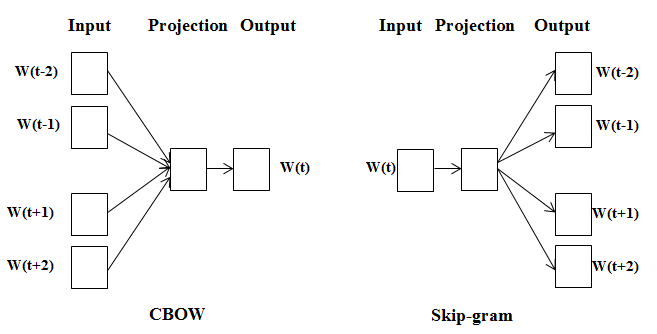
\includegraphics[width=0.75\linewidth]{new figures/Word2Vec.png}
    \caption{Word2Vec Architectures}
    \label{fig:word2vec}
\end{figure}


\subsubsection{GloVe: Global Vectors for Word Representation}
GloVe constructs word embeddings by factorizing a global word–word co-occurrence matrix derived from a corpus. The co-occurrence matrix records how frequently word appears in the context of word across the entire corpus. GloVe minimizes a weighted least-squares objective that forces the dot product of two word vectors to approximate the logarithm of their co-occurrence count. This approach combines the benefits of global matrix factorization methods with local context window methods. The resulting embeddings reflect both global statistics and local context, enabling robust representation for downstream tasks such as sentiment analysis or text classification
\subsubsection{FastText}
FastText extends Word2Vec by representing each word as a bag of character n-grams (e.g., “apple” ->{“<ap”, “pp”, “pl”, “le”>”}). During training, each n-gram is assigned an embedding, and a word’s embedding is obtained by summing the embeddings of its constituent n-grams. This subword modeling enables FastText to generate meaningful embeddings for rare or out-of-vocabulary words based on their morphological components. Both CBOW and Skip-Gram architectures are supported, with the same training objectives as Word2Vec. FastText embeddings are best suited for .

\subsubsection{Bert Embeddings}
BERT (Bidirectional Encoder Representations from Transformers) produces contextualized embeddings by passing text through multiple layers of self-attention. Each token’s embedding is computed with full awareness of both its left and right context. Input text is first tokenized using WordPiece subword segmentation, then encoded with positional and segment embeddings. The final hidden states of the transformer layers serve as rich, context-dependent representations for each token. Sentence or document-level embeddings can be derived by pooling strategies (e.g., mean pooling or using the [CLS] token) for downstream classification tasks.

\subsection{Machine learning} Machine learning models are fundamental to text classification tasks in NLP, where the goal is to assign predefined labels to textual inputs. Traditional models such as Naïve Bayes, Support Vector Machines (SVM) and Logistic Regression have been widely used due to their simplicity and effectiveness with feature-engineered representations like TF-IDF. These models rely on statistical patterns in the text and perform well on structured and moderately sized datasets. Ensemble methods, such as Random Forests, further enhance classification accuracy by combining the predictions of multiple base learners. Despite their limitations in capturing complex linguistic structures, these models remain competitive in many practical applications due to their simplicity compared to deep learning architectures.

\subsubsection{Logistic Regression} Logistic regression is a linear classifier that predicts the probability of a categorical outcome. It applies the sigmoid function to map linear combinations of input features into probability values between 0 and 1. In the context of this study, it was used as a baseline model for multi-class classification (Normal, BPD, Inconclusive), benefiting from its simplicity and interpretability.

\subsubsection{Linear Support Vector Machine} Linear SVM is a powerful classifier that aims to find the optimal hyperplane that maximizes the margin between classes. The linear SVM was used for text classification due to its effectiveness in high-dimensional spaces and its ability to handle sparse text data.

\subsubsection{Multinomial Naive Bayes}  Multinomial naive bayes is a probabilistic classifier based on Bayes' theorem and assumes feature independence. It is particularly well-suited for text classification where input features represent term frequencies or TF-IDF values.

\subsubsection{Decision Tree} Decision tree is a non-linear model that recursively splits the data based on feature thresholds to form a tree-like structure. It is highly interpretable and can handle both numerical and categorical features.

\subsubsection{Random Forest} Random forest is an ensemble learning method that constructs a multitude of decision trees and outputs the mode of their predictions (classification) or mean (regression). It introduces randomness via bootstrapped sampling and feature selection at each split.

\subsubsection{XGBoost} Extreme Gradient Boosting or XGBoost is a highly efficient and scalable implementation of gradient boosting decision trees. It builds trees sequentially, where each new tree attempts to correct the errors of the previous ones.

\subsubsection{AdaBoost} Adaptive Boosting combines multiple weak learners (typically shallow decision trees) into a strong classifier by focusing more on instances misclassified by previous models. Each subsequent model gives more weight to difficult samples.
    
\subsubsection{LightGBM} is a gradient boosting framework optimized for performance and speed. It uses a leaf-wise tree growth strategy and supports categorical features natively.

\subsection{Deep Learning Models}
To capture temporal dependencies, semantic patterns, and contextual nuances in user responses, several deep learning architectures were employed. These models are particularly effective in modeling sequential data, making them suitable for natural language processing tasks such as mental health classification.

\subsubsection{LSTM} Long Short-Term Memory or LSTM is a type of Recurrent Neural Network (RNN) designed to learn long-term dependencies in sequential data. Unlike standard RNNs, LSTMs mitigate the vanishing gradient problem by using a memory cell and three gates—input, forget, and output—which control information flow.

\subsubsection{GRU} Gated Recurrent Unit is a simplified version of LSTM that uses only two gates: update and reset. It has fewer parameters than LSTM, making it faster to train while retaining similar performance.

\subsubsection{BiLSTM} Bidirectional LSTM extends the LSTM architecture by processing the input sequence in both forward and backward directions. This helps the model understand context from both past and future tokens.

\subsubsection{BiGRU} Bidirectional GRU or BiGRU is the bidirectional counterpart of GRU, capable of processing input sequences from both directions. It combines the efficiency of GRU with the bidirectional contextual awareness of BiLSTM.

\subsubsection{CNN} CNN or Convolutional Neural Network are traditionally used in computer vision, they are also effective in text classification by capturing local patterns in a sentence (e.g., key phrases or n-grams). CNNs use filters to slide over word embeddings to extract hierarchical features.


\subsection{Oversampling Technique}
Oversampling is a technique used to address class imbalance in datasets, particularly when one or more classes (minority classes) have significantly fewer samples than the majority class. This imbalance can negatively impact model performance, especially for detecting minority class instances. Oversampling increases the number of samples in the minority class to balance the dataset.
\subsubsection{SMOTE} Synthetic Minority Over-sampling Technique or SMOTE generates synthetic samples for the minority class by interpolating between existing minority instances and their nearest neighbors. This helps balance the dataset without duplicating existing samples, improving model performance on underrepresented classes.

\subsubsection{ADASYN} Adaptive Synthetic Sampling or ADASYN builds on SMOTE by adaptively generating more synthetic data for harder-to-learn minority class samples—i.e., those that are more difficult to classify. It focuses on areas where class imbalance has a greater impact, making the classifier more robust.

\subsection{Explainable AI}
Explainable Artificial Intelligence (XAI) refers to a set of methods and techniques that make the decisions and predictions of AI systems understandable and transparent to humans. Unlike traditional black-box models which provide little to no insight into how outputs are generated, XAI aims to clarify how and why a model arrives at a particular decision. This is especially important in critical fields where trust, accountability, and interpretability are essential. XAI techniques help identify which features influenced a model’s decision, highlight potential biases, and ensure that predictions align with human reasoning and domain knowledge. Ultimately, XAI bridges the gap between complex machine learning models and human users, promoting ethical AI use and increasing confidence in AI-driven outcomes.One of the model for xai is \textbf{LIME}.
\subsubsection{LIME}
LIME (Local Interpretable Model-agnostic Explanations) is an Explainable AI technique that helps interpret complex machine learning models by providing local human-understandable explanations for individual predictions. For text data, LIME works by slightly altering the input (e.g., removing or changing words) and observing how these changes affect the model’s output. It then builds a simple, interpretable model around the specific prediction to identify which words contributed most to the final decision.This makes LIME especially useful for understanding and validating model behavior in sensitive applications like mental health diagnosis.
\begin{figure}[H]
    \centering
    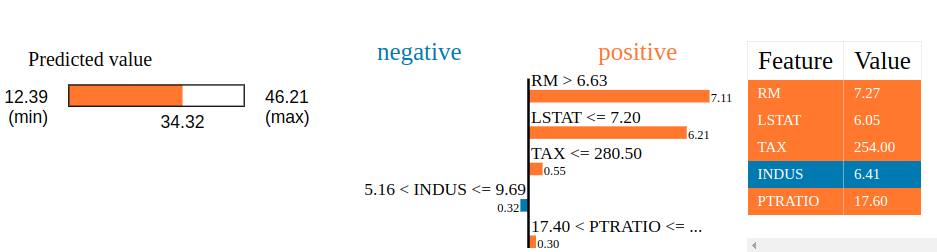
\includegraphics[width=0.75\linewidth]{XAI.png}
    \caption{XAI Output}
    \label{fig:XAI}
\end{figure}



\section{Related Works}
 The existing literature on detecting personality disorders or mental health illnesses in general primarily emphasizes analyzing social media texts. Recent studies have successfully detected personality disorders by analyzing social media texts through machine learning or deep learning architectures \cite{jain2024text} \cite{ellouze2022deep} \cite{singh2020framework} \cite{ellouze2022hybrid}, where only one study accomplished multi-class classification and used large language models \cite{jain2024text}. However, there are few real-world applications of classifying social media text, as an individual cannot be conclusively diagnosed based on their social media text. Furthermore, a person cannot be informed about the presence of personality disorder symptoms through social media text analysis, as a person's consent must be taken beforehand to analyze their social media content due to privacy concerns. A different approach was employed in \cite{khazbak2021mindtime}, where a diary application was developed to analyze users' daily notes on events, experiences, thoughts and emotions to detect symptoms of borderline personality disorder using Naive Bayes, SVM, KNN and LSTM classifiers. Users of the app, however, cannot be definitively diagnosed from their notes only. Previous research has also encountered challenges in obtaining annotated text datasets for mental illness detection, as expert assistance is essential for accurately labeling mental health-related data.
    
Earlier studies have also made efforts to detect mental illnesses in general from social media text analysis \cite{dinu2021automatic} \cite{jiang-etal-2020-detection} \cite{yang2024mentallama} \cite{vajre2021psychbert} \cite{xu2024mental} \cite{martinez2022early} and have similarly faced challenges in obtaining annotated text datasets for diagnosing mental illnesses. In addition, social media text is inadequate to diagnose patients definitively as discussed before. It is worth noting, that fine-tuning LLMs boosts performance and accuracy \cite{xu2024mental}. Previous studies have utilized large language models, especially encoder-only models, in mental health classification tasks \cite{jain2024text} \cite{dinu2021automatic} \cite{jiang-etal-2020-detection} \cite{yang2024mentallama} \cite{vajre2021psychbert} \cite{xu2024mental} \cite{martinez2022early} \cite{suicidalideationtransformers2020}, but further research is required to determine efficacy of these models in clinical QnA classification in the mental health domain.

Previous research has noted challenges in mental illness detection using natural language processing, such as real-world applicability, inadequacy of expert annotated dataset and the potential limitation of focusing on social media \cite{montejo2024survey} \cite{zhang2022natural} \cite{ellouze2024artificial} \cite{greco2023transformer}. Hence, more research is required to overcome these limitations as well.

Personality disorder identification is crucial, however, earlier studies have not explored how to give individuals a preliminary diagnosis based on their texts. Social media text analysis for personality disorder detection has few real-world applications, as users cannot be conclusively diagnosed based on their social media texts only.
To the best of our knowledge, the existing literature has mainly used social media text datasets for training models to detect personality disorders \cite{jain2024text} \cite{ellouze2022deep} \cite{singh2020framework} \cite{ellouze2022hybrid}. However, psychiatrists and psychologists diagnose patients through question-answer sessions, not through social media analysis. Without a definitive diagnosis, individuals are not able to seek appropriate help or take steps to address the symptoms of the disorder. For this reason, it is imperative to develop a question-and-answer text dataset to match the format of personality disorder diagnosis. 

Little is known about how existing models trained on publicly available mental health datasets, created from social media or online forums, would perform in clinical environments, where texts are in a question-answer format. Training machine learning, deep learning and large language models using an annotated question-and-answer dataset is crucial for use in a clinical setting. To achieve this, a multidisciplinary study is required to develop an annotated question-and-answer dataset, created in collaboration with psychiatrists and psychologists. This dataset can then be used to train, evaluate and compare machine learning, deep learning and large language models for preliminary screening of borderline personality disorder, intended for use in a clinical context.



\section{Critical Summary}
 The existing research mainly focuses on social media text for personality disorder or mental health disorder detection in general. However, social media text is not appropriate for preliminary screening of mental health disorders. To the best of our knowledge, a QnA classification dataset for mental disorder screening, specifically for borderline personality disorder screening has not yet been created. The QnA format of mental illness remains an avenue to be investigated. Furthermore, existing BPD screening tools rely on dichotomous questions and Likert scales, which have significant disadvantages, such as reduced data accuracy, lack of response depth and limited analysis. Therefore, an NLP-based screening tool that incorporates LLM-driven QnA classification and explainable AI would be a significant advancement in the field of AI-based mental disorder detection.


\endinput

